% Options for packages loaded elsewhere
\PassOptionsToPackage{unicode}{hyperref}
\PassOptionsToPackage{hyphens}{url}
\PassOptionsToPackage{dvipsnames,svgnames,x11names}{xcolor}
%
\documentclass[
  letterpaper,
  DIV=11,
  numbers=noendperiod]{scrartcl}

\usepackage{amsmath,amssymb}
\usepackage{iftex}
\ifPDFTeX
  \usepackage[T1]{fontenc}
  \usepackage[utf8]{inputenc}
  \usepackage{textcomp} % provide euro and other symbols
\else % if luatex or xetex
  \usepackage{unicode-math}
  \defaultfontfeatures{Scale=MatchLowercase}
  \defaultfontfeatures[\rmfamily]{Ligatures=TeX,Scale=1}
\fi
\usepackage{lmodern}
\ifPDFTeX\else  
    % xetex/luatex font selection
\fi
% Use upquote if available, for straight quotes in verbatim environments
\IfFileExists{upquote.sty}{\usepackage{upquote}}{}
\IfFileExists{microtype.sty}{% use microtype if available
  \usepackage[]{microtype}
  \UseMicrotypeSet[protrusion]{basicmath} % disable protrusion for tt fonts
}{}
\makeatletter
\@ifundefined{KOMAClassName}{% if non-KOMA class
  \IfFileExists{parskip.sty}{%
    \usepackage{parskip}
  }{% else
    \setlength{\parindent}{0pt}
    \setlength{\parskip}{6pt plus 2pt minus 1pt}}
}{% if KOMA class
  \KOMAoptions{parskip=half}}
\makeatother
\usepackage{xcolor}
\setlength{\emergencystretch}{3em} % prevent overfull lines
\setcounter{secnumdepth}{-\maxdimen} % remove section numbering
% Make \paragraph and \subparagraph free-standing
\makeatletter
\ifx\paragraph\undefined\else
  \let\oldparagraph\paragraph
  \renewcommand{\paragraph}{
    \@ifstar
      \xxxParagraphStar
      \xxxParagraphNoStar
  }
  \newcommand{\xxxParagraphStar}[1]{\oldparagraph*{#1}\mbox{}}
  \newcommand{\xxxParagraphNoStar}[1]{\oldparagraph{#1}\mbox{}}
\fi
\ifx\subparagraph\undefined\else
  \let\oldsubparagraph\subparagraph
  \renewcommand{\subparagraph}{
    \@ifstar
      \xxxSubParagraphStar
      \xxxSubParagraphNoStar
  }
  \newcommand{\xxxSubParagraphStar}[1]{\oldsubparagraph*{#1}\mbox{}}
  \newcommand{\xxxSubParagraphNoStar}[1]{\oldsubparagraph{#1}\mbox{}}
\fi
\makeatother

\usepackage{color}
\usepackage{fancyvrb}
\newcommand{\VerbBar}{|}
\newcommand{\VERB}{\Verb[commandchars=\\\{\}]}
\DefineVerbatimEnvironment{Highlighting}{Verbatim}{commandchars=\\\{\}}
% Add ',fontsize=\small' for more characters per line
\usepackage{framed}
\definecolor{shadecolor}{RGB}{241,243,245}
\newenvironment{Shaded}{\begin{snugshade}}{\end{snugshade}}
\newcommand{\AlertTok}[1]{\textcolor[rgb]{0.68,0.00,0.00}{#1}}
\newcommand{\AnnotationTok}[1]{\textcolor[rgb]{0.37,0.37,0.37}{#1}}
\newcommand{\AttributeTok}[1]{\textcolor[rgb]{0.40,0.45,0.13}{#1}}
\newcommand{\BaseNTok}[1]{\textcolor[rgb]{0.68,0.00,0.00}{#1}}
\newcommand{\BuiltInTok}[1]{\textcolor[rgb]{0.00,0.23,0.31}{#1}}
\newcommand{\CharTok}[1]{\textcolor[rgb]{0.13,0.47,0.30}{#1}}
\newcommand{\CommentTok}[1]{\textcolor[rgb]{0.37,0.37,0.37}{#1}}
\newcommand{\CommentVarTok}[1]{\textcolor[rgb]{0.37,0.37,0.37}{\textit{#1}}}
\newcommand{\ConstantTok}[1]{\textcolor[rgb]{0.56,0.35,0.01}{#1}}
\newcommand{\ControlFlowTok}[1]{\textcolor[rgb]{0.00,0.23,0.31}{\textbf{#1}}}
\newcommand{\DataTypeTok}[1]{\textcolor[rgb]{0.68,0.00,0.00}{#1}}
\newcommand{\DecValTok}[1]{\textcolor[rgb]{0.68,0.00,0.00}{#1}}
\newcommand{\DocumentationTok}[1]{\textcolor[rgb]{0.37,0.37,0.37}{\textit{#1}}}
\newcommand{\ErrorTok}[1]{\textcolor[rgb]{0.68,0.00,0.00}{#1}}
\newcommand{\ExtensionTok}[1]{\textcolor[rgb]{0.00,0.23,0.31}{#1}}
\newcommand{\FloatTok}[1]{\textcolor[rgb]{0.68,0.00,0.00}{#1}}
\newcommand{\FunctionTok}[1]{\textcolor[rgb]{0.28,0.35,0.67}{#1}}
\newcommand{\ImportTok}[1]{\textcolor[rgb]{0.00,0.46,0.62}{#1}}
\newcommand{\InformationTok}[1]{\textcolor[rgb]{0.37,0.37,0.37}{#1}}
\newcommand{\KeywordTok}[1]{\textcolor[rgb]{0.00,0.23,0.31}{\textbf{#1}}}
\newcommand{\NormalTok}[1]{\textcolor[rgb]{0.00,0.23,0.31}{#1}}
\newcommand{\OperatorTok}[1]{\textcolor[rgb]{0.37,0.37,0.37}{#1}}
\newcommand{\OtherTok}[1]{\textcolor[rgb]{0.00,0.23,0.31}{#1}}
\newcommand{\PreprocessorTok}[1]{\textcolor[rgb]{0.68,0.00,0.00}{#1}}
\newcommand{\RegionMarkerTok}[1]{\textcolor[rgb]{0.00,0.23,0.31}{#1}}
\newcommand{\SpecialCharTok}[1]{\textcolor[rgb]{0.37,0.37,0.37}{#1}}
\newcommand{\SpecialStringTok}[1]{\textcolor[rgb]{0.13,0.47,0.30}{#1}}
\newcommand{\StringTok}[1]{\textcolor[rgb]{0.13,0.47,0.30}{#1}}
\newcommand{\VariableTok}[1]{\textcolor[rgb]{0.07,0.07,0.07}{#1}}
\newcommand{\VerbatimStringTok}[1]{\textcolor[rgb]{0.13,0.47,0.30}{#1}}
\newcommand{\WarningTok}[1]{\textcolor[rgb]{0.37,0.37,0.37}{\textit{#1}}}

\providecommand{\tightlist}{%
  \setlength{\itemsep}{0pt}\setlength{\parskip}{0pt}}\usepackage{longtable,booktabs,array}
\usepackage{calc} % for calculating minipage widths
% Correct order of tables after \paragraph or \subparagraph
\usepackage{etoolbox}
\makeatletter
\patchcmd\longtable{\par}{\if@noskipsec\mbox{}\fi\par}{}{}
\makeatother
% Allow footnotes in longtable head/foot
\IfFileExists{footnotehyper.sty}{\usepackage{footnotehyper}}{\usepackage{footnote}}
\makesavenoteenv{longtable}
\usepackage{graphicx}
\makeatletter
\def\maxwidth{\ifdim\Gin@nat@width>\linewidth\linewidth\else\Gin@nat@width\fi}
\def\maxheight{\ifdim\Gin@nat@height>\textheight\textheight\else\Gin@nat@height\fi}
\makeatother
% Scale images if necessary, so that they will not overflow the page
% margins by default, and it is still possible to overwrite the defaults
% using explicit options in \includegraphics[width, height, ...]{}
\setkeys{Gin}{width=\maxwidth,height=\maxheight,keepaspectratio}
% Set default figure placement to htbp
\makeatletter
\def\fps@figure{htbp}
\makeatother

\KOMAoption{captions}{tableheading}
\makeatletter
\@ifpackageloaded{caption}{}{\usepackage{caption}}
\AtBeginDocument{%
\ifdefined\contentsname
  \renewcommand*\contentsname{Table of contents}
\else
  \newcommand\contentsname{Table of contents}
\fi
\ifdefined\listfigurename
  \renewcommand*\listfigurename{List of Figures}
\else
  \newcommand\listfigurename{List of Figures}
\fi
\ifdefined\listtablename
  \renewcommand*\listtablename{List of Tables}
\else
  \newcommand\listtablename{List of Tables}
\fi
\ifdefined\figurename
  \renewcommand*\figurename{Figure}
\else
  \newcommand\figurename{Figure}
\fi
\ifdefined\tablename
  \renewcommand*\tablename{Table}
\else
  \newcommand\tablename{Table}
\fi
}
\@ifpackageloaded{float}{}{\usepackage{float}}
\floatstyle{ruled}
\@ifundefined{c@chapter}{\newfloat{codelisting}{h}{lop}}{\newfloat{codelisting}{h}{lop}[chapter]}
\floatname{codelisting}{Listing}
\newcommand*\listoflistings{\listof{codelisting}{List of Listings}}
\makeatother
\makeatletter
\makeatother
\makeatletter
\@ifpackageloaded{caption}{}{\usepackage{caption}}
\@ifpackageloaded{subcaption}{}{\usepackage{subcaption}}
\makeatother

\ifLuaTeX
  \usepackage{selnolig}  % disable illegal ligatures
\fi
\usepackage{bookmark}

\IfFileExists{xurl.sty}{\usepackage{xurl}}{} % add URL line breaks if available
\urlstyle{same} % disable monospaced font for URLs
\hypersetup{
  pdftitle={Assignment 2},
  pdfauthor={Group 2},
  colorlinks=true,
  linkcolor={blue},
  filecolor={Maroon},
  citecolor={Blue},
  urlcolor={Blue},
  pdfcreator={LaTeX via pandoc}}


\title{Assignment 2}
\author{Group 2}
\date{2025-03-13}

\begin{document}
\maketitle


\section{We will explore the data we scraped to determine next steps for
analysis.}\label{we-will-explore-the-data-we-scraped-to-determine-next-steps-for-analysis.}

\begin{enumerate}
\def\labelenumi{\arabic{enumi}.}
\tightlist
\item
  Read in data from github, and tidy it to continue processing.
\end{enumerate}

\begin{Shaded}
\begin{Highlighting}[]
\CommentTok{\# posts data}
\NormalTok{reddit\_posts }\OtherTok{\textless{}{-}} \FunctionTok{read\_xlsx}\NormalTok{(}
  \CommentTok{\# "\textasciitilde{}/repos/SURV622\_Assignment/data/posts\_data\_clean.xlsx") |\textgreater{} path for Kevin}
  \StringTok{"\textasciitilde{}/Desktop/UMICH/SURV622\_Assignment/data/posts\_data\_clean.xlsx"}\NormalTok{) }\SpecialCharTok{|\textgreater{}} \CommentTok{\# path for Felix}
  \FunctionTok{mutate}\NormalTok{(}\AttributeTok{date\_utc =} \FunctionTok{ymd}\NormalTok{(date\_utc)) }\SpecialCharTok{|\textgreater{}} 
  \CommentTok{\# remove variables not needed}
  \CommentTok{\# select({-}timestamp)}
  \FunctionTok{mutate}\NormalTok{(}
    \CommentTok{\# Convert timestamp to POSIXct format}
    \AttributeTok{timestamp =} \FunctionTok{as.POSIXct}\NormalTok{(timestamp, }\AttributeTok{origin =} \StringTok{"1970{-}01{-}01"}\NormalTok{, }\AttributeTok{tz =} \StringTok{"UTC"}\NormalTok{),}
    
    \CommentTok{\# Extract time of day (you can adjust the format as needed)}
    \AttributeTok{time\_of\_day =} \FunctionTok{format}\NormalTok{(timestamp, }\StringTok{"\%H:\%M:\%S"}\NormalTok{)}
\NormalTok{  )}


\CommentTok{\# comments data}
\NormalTok{reddit\_comment }\OtherTok{\textless{}{-}} \FunctionTok{read\_xlsx}\NormalTok{(}
  \CommentTok{\# "\textasciitilde{}/repos/SURV622\_Assignment/data/comments\_data\_clean.xlsx") |\textgreater{} Kevin\textquotesingle{}s path}
  \StringTok{"\textasciitilde{}/Desktop/UMICH/SURV622\_Assignment/data/comments\_data\_clean.xlsx"}\NormalTok{) }\SpecialCharTok{|\textgreater{}} \CommentTok{\# Felix\textquotesingle{}s path}
    \FunctionTok{mutate}\NormalTok{(}\AttributeTok{date\_utc =} \FunctionTok{ymd}\NormalTok{(date\_utc)) }\SpecialCharTok{|\textgreater{}} 
  \CommentTok{\# great unique post id}
  \FunctionTok{arrange}\NormalTok{(date\_utc) }\SpecialCharTok{|\textgreater{}} 
  \FunctionTok{group\_by}\NormalTok{(url) }\SpecialCharTok{|\textgreater{}} 
  \FunctionTok{mutate}\NormalTok{(}\AttributeTok{post\_id =} \FunctionTok{cur\_group\_id}\NormalTok{()) }\SpecialCharTok{|\textgreater{}} 
  \FunctionTok{ungroup}\NormalTok{() }\SpecialCharTok{|\textgreater{}} 
  \CommentTok{\# remove variables not needed}
  \FunctionTok{mutate}\NormalTok{(}
    \CommentTok{\# Convert timestamp to POSIXct format}
    \AttributeTok{timestamp =} \FunctionTok{as.POSIXct}\NormalTok{(timestamp, }\AttributeTok{origin =} \StringTok{"1970{-}01{-}01"}\NormalTok{, }\AttributeTok{tz =} \StringTok{"UTC"}\NormalTok{),}
    
    \CommentTok{\# Extract time of day (you can adjust the format as needed)}
    \AttributeTok{time\_of\_day =} \FunctionTok{format}\NormalTok{(timestamp, }\StringTok{"\%H:\%M:\%S"}\NormalTok{)}
\NormalTok{  ) }\SpecialCharTok{|\textgreater{}}
  \FunctionTok{select}\NormalTok{(}\SpecialCharTok{{-}}\NormalTok{author, }\SpecialCharTok{{-}}\NormalTok{comment\_id) }


\CommentTok{\# id url group IDs to the posts data}
\NormalTok{reddit\_posts\_2 }\OtherTok{\textless{}{-}}\NormalTok{ reddit\_posts }\SpecialCharTok{|\textgreater{}} 
  \FunctionTok{semi\_join}\NormalTok{(reddit\_comment }\SpecialCharTok{|\textgreater{}} \FunctionTok{select}\NormalTok{(url, post\_id)) }
\end{Highlighting}
\end{Shaded}

\subsubsection{The strings we will be processing sometimes have special
characters, numbers, brackets. We need to clean these string for
processing.}\label{the-strings-we-will-be-processing-sometimes-have-special-characters-numbers-brackets.-we-need-to-clean-these-string-for-processing.}

\begin{itemize}
\tightlist
\item
  We can use the fedmatch::clean\_strings() function to tidy up the
  text. The following is an example of what will be cleaned.
\end{itemize}

\begin{Shaded}
\begin{Highlighting}[]
\CommentTok{\# print example of posts}
\NormalTok{reddit\_posts }\SpecialCharTok{|\textgreater{}} 
  \FunctionTok{slice}\NormalTok{(}\DecValTok{10}\SpecialCharTok{:}\DecValTok{15}\NormalTok{) }\SpecialCharTok{|\textgreater{}} 
  \FunctionTok{select}\NormalTok{(text) }
\end{Highlighting}
\end{Shaded}

\begin{verbatim}
# A tibble: 6 x 1
  text                                                                          
  <chr>                                                                         
1 <NA>                                                                          
2 <NA>                                                                          
3 <NA>                                                                          
4 <NA>                                                                          
5 <NA>                                                                          
6 commerce secretary howard lutnick said sunday that government spending could ~
\end{verbatim}

\begin{Shaded}
\begin{Highlighting}[]
\CommentTok{\# clean posts}
\NormalTok{reddit\_posts }\SpecialCharTok{|\textgreater{}} 
  \FunctionTok{slice}\NormalTok{(}\DecValTok{10}\SpecialCharTok{:}\DecValTok{15}\NormalTok{) }\SpecialCharTok{|\textgreater{}} 
  \FunctionTok{mutate}\NormalTok{(}\AttributeTok{text =} \FunctionTok{clean\_strings}\NormalTok{(text)) }\SpecialCharTok{|\textgreater{}} 
  \FunctionTok{select}\NormalTok{(text) }
\end{Highlighting}
\end{Shaded}

\begin{verbatim}
# A tibble: 6 x 1
  text                                                                          
  <chr>                                                                         
1 <NA>                                                                          
2 <NA>                                                                          
3 <NA>                                                                          
4 <NA>                                                                          
5 <NA>                                                                          
6 commerce secretary howard lutnick said sunday that government spending could ~
\end{verbatim}

\begin{itemize}
\tightlist
\item
  Clean posts and comment strings.
\end{itemize}

\begin{Shaded}
\begin{Highlighting}[]
\NormalTok{reddit\_posts }\OtherTok{\textless{}{-}}\NormalTok{ reddit\_posts }\SpecialCharTok{|\textgreater{}} 
  \FunctionTok{mutate}\NormalTok{(}\AttributeTok{text =} \FunctionTok{clean\_strings}\NormalTok{(text))}

\NormalTok{reddit\_comment }\OtherTok{\textless{}{-}}\NormalTok{ reddit\_comment }\SpecialCharTok{|\textgreater{}} 
  \FunctionTok{mutate}\NormalTok{(}\AttributeTok{comment =} \FunctionTok{clean\_strings}\NormalTok{(comment))}

\NormalTok{reddit\_posts\_2 }\OtherTok{\textless{}{-}}\NormalTok{ reddit\_posts\_2 }\SpecialCharTok{|\textgreater{}} 
  \FunctionTok{mutate}\NormalTok{(}\AttributeTok{text=}\FunctionTok{clean\_strings}\NormalTok{(text))}
\end{Highlighting}
\end{Shaded}

\hfill\break

\subsubsection{We can now begin to explore the data. First we explore
the
posts.}\label{we-can-now-begin-to-explore-the-data.-first-we-explore-the-posts.}

\begin{Shaded}
\begin{Highlighting}[]
\NormalTok{  reddit\_posts }\SpecialCharTok{|\textgreater{}}
  \FunctionTok{slice}\NormalTok{(}\DecValTok{364}\NormalTok{) }\SpecialCharTok{|\textgreater{}} 
  \FunctionTok{pull}\NormalTok{(text) }
\end{Highlighting}
\end{Shaded}

{[}1{]} ``hello all so i recently took the deferred resignation i was
working at the va and my job was not exempt i did not trust that my job
was safe even after coming off probation the day the fork in the road
came out i took the resignation and my last day was february 28 before i
started i was in the cwt program compensated work therapy i once again
have an opportunity to get back into the program i know we are allowed
to work while on the resignation but am i able to do the cwt because
both checks would be federal payments i don t want to lose out on the
resignation benefits just to make 12 hr but working does help me mental
health and give me a purpose any insight would be greatly appreciated''

\subsection{How many posts were collected in total and by day? How many
posts after data cleaning? Is there a pattern with respect to the time
of day or day of week when posts were created? Is there a relationship
between events and frequency of
tweets?}\label{how-many-posts-were-collected-in-total-and-by-day-how-many-posts-after-data-cleaning-is-there-a-pattern-with-respect-to-the-time-of-day-or-day-of-week-when-posts-were-created-is-there-a-relationship-between-events-and-frequency-of-tweets}

\begin{Shaded}
\begin{Highlighting}[]
\CommentTok{\# number of total posts}
\NormalTok{totalposts }\OtherTok{\textless{}{-}}\NormalTok{ reddit\_posts }\SpecialCharTok{\%\textgreater{}\%}
  \FunctionTok{summarize}\NormalTok{(}
    \AttributeTok{TotalPosts =} \FunctionTok{n}\NormalTok{()}
\NormalTok{  )}
\NormalTok{knitr}\SpecialCharTok{::}\FunctionTok{kable}\NormalTok{(totalposts)}
\end{Highlighting}
\end{Shaded}

\begin{longtable}[]{@{}r@{}}
\toprule\noalign{}
TotalPosts \\
\midrule\noalign{}
\endhead
\bottomrule\noalign{}
\endlastfoot
557 \\
\end{longtable}

\begin{Shaded}
\begin{Highlighting}[]
\CommentTok{\# number of posts by day}
\NormalTok{byday\_posts }\OtherTok{\textless{}{-}}\NormalTok{ reddit\_posts }\SpecialCharTok{\%\textgreater{}\%}
  \FunctionTok{group\_by}\NormalTok{(date\_utc) }\SpecialCharTok{\%\textgreater{}\%}
  \FunctionTok{summarize}\NormalTok{(}
    \AttributeTok{total =} \FunctionTok{n}\NormalTok{()}
\NormalTok{  )}

\CommentTok{\# plot}
\FunctionTok{ggplot}\NormalTok{(byday\_posts, }\FunctionTok{aes}\NormalTok{(}\AttributeTok{x =}\NormalTok{ date\_utc, }\AttributeTok{y =}\NormalTok{ total)) }\SpecialCharTok{+} 
  \FunctionTok{geom\_point}\NormalTok{(}\AttributeTok{color =} \StringTok{"blue"}\NormalTok{, }\AttributeTok{size =} \DecValTok{3}\NormalTok{) }\SpecialCharTok{+}  
  \FunctionTok{geom\_line}\NormalTok{(}\AttributeTok{color =} \StringTok{"steelblue"}\NormalTok{, }\AttributeTok{linewidth =} \DecValTok{1}\NormalTok{) }\SpecialCharTok{+}  
  \FunctionTok{labs}\NormalTok{(}
    \AttributeTok{title =} \StringTok{"Total Number of Posts per Day"}\NormalTok{,}
    \AttributeTok{x =} \StringTok{"Day"}\NormalTok{,}
    \AttributeTok{y =} \StringTok{"Total Number of Posts"}
\NormalTok{  ) }\SpecialCharTok{+}
  \FunctionTok{theme\_minimal}\NormalTok{()}
\end{Highlighting}
\end{Shaded}

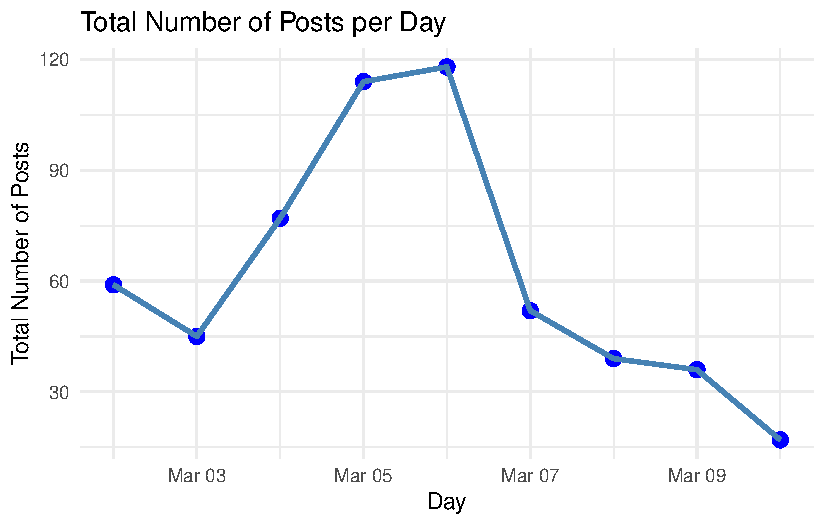
\includegraphics{Reddit_eda_files/figure-pdf/unnamed-chunk-5-1.pdf}

\begin{Shaded}
\begin{Highlighting}[]
\CommentTok{\# number of total comments}
\NormalTok{totalcomments }\OtherTok{\textless{}{-}}\NormalTok{ reddit\_comment }\SpecialCharTok{\%\textgreater{}\%}
  \FunctionTok{summarize}\NormalTok{(}
    \AttributeTok{TotalPosts =} \FunctionTok{n}\NormalTok{()}
\NormalTok{  )}
\NormalTok{knitr}\SpecialCharTok{::}\FunctionTok{kable}\NormalTok{(totalcomments)}
\end{Highlighting}
\end{Shaded}

\begin{longtable}[]{@{}r@{}}
\toprule\noalign{}
TotalPosts \\
\midrule\noalign{}
\endhead
\bottomrule\noalign{}
\endlastfoot
12492 \\
\end{longtable}

\begin{Shaded}
\begin{Highlighting}[]
\CommentTok{\# number of comments by day}
\NormalTok{byday\_comments }\OtherTok{\textless{}{-}}\NormalTok{ reddit\_comment }\SpecialCharTok{\%\textgreater{}\%}
  \FunctionTok{group\_by}\NormalTok{(date\_utc) }\SpecialCharTok{\%\textgreater{}\%}
  \FunctionTok{summarize}\NormalTok{(}
    \AttributeTok{total =} \FunctionTok{n}\NormalTok{()}
\NormalTok{  )}

\CommentTok{\# plot}
\FunctionTok{ggplot}\NormalTok{(byday\_comments, }\FunctionTok{aes}\NormalTok{(}\AttributeTok{x =}\NormalTok{ date\_utc, }\AttributeTok{y =}\NormalTok{ total)) }\SpecialCharTok{+} 
  \FunctionTok{geom\_point}\NormalTok{(}\AttributeTok{color =} \StringTok{"green"}\NormalTok{, }\AttributeTok{size =} \DecValTok{3}\NormalTok{) }\SpecialCharTok{+}  
  \FunctionTok{geom\_line}\NormalTok{(}\AttributeTok{color =} \StringTok{"lightgreen"}\NormalTok{, }\AttributeTok{linewidth =} \DecValTok{1}\NormalTok{) }\SpecialCharTok{+}
  \FunctionTok{labs}\NormalTok{(}
    \AttributeTok{title =} \StringTok{"Total Number of Posts per Day"}\NormalTok{,}
    \AttributeTok{x =} \StringTok{"Day"}\NormalTok{,}
    \AttributeTok{y =} \StringTok{"Total Number of Posts"}
\NormalTok{  ) }\SpecialCharTok{+}
  \FunctionTok{theme\_minimal}\NormalTok{()}
\end{Highlighting}
\end{Shaded}

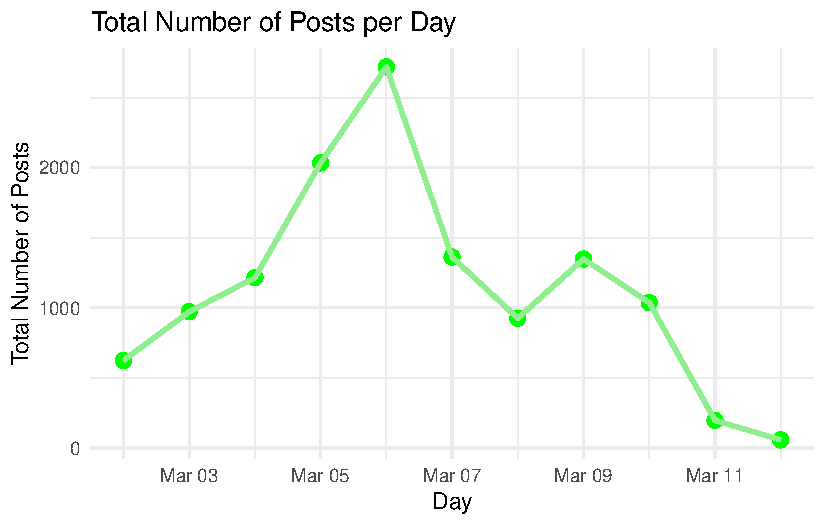
\includegraphics{Reddit_eda_files/figure-pdf/unnamed-chunk-5-2.pdf}

There appears to be a noticeable peak in activity during the middle of
the week. However, we don't have enough data to conclusively say it's
due to the day of the week itself. It's more likely that these spikes
are linked to specific events that occurred on those days, which sparked
conversations.

The two peaks in our graph could be attributed to two major news
stories. On March 5, Elon Musk made a statement about wanting to ``save
Western civilization from empathy,'' and on March 6, there were reports
that President Trump was limiting Musk's authority due to backlash over
cuts to DOGE. These events likely had a significant impact on the volume
of Reddit posts related to Elon Musk and DOGE, driving the observed
spikes in activity.

\begin{Shaded}
\begin{Highlighting}[]
\CommentTok{\# Number of posts by time of day (hour)}
\NormalTok{byhour\_posts }\OtherTok{\textless{}{-}}\NormalTok{ reddit\_posts }\SpecialCharTok{\%\textgreater{}\%}
  \FunctionTok{mutate}\NormalTok{(}\AttributeTok{hour\_of\_day =} \FunctionTok{hour}\NormalTok{(timestamp)) }\SpecialCharTok{\%\textgreater{}\%}
  \FunctionTok{group\_by}\NormalTok{(hour\_of\_day) }\SpecialCharTok{\%\textgreater{}\%}
  \FunctionTok{summarize}\NormalTok{(}\AttributeTok{total =} \FunctionTok{n}\NormalTok{())}

\CommentTok{\# Plot number of posts by hour of day}
\FunctionTok{ggplot}\NormalTok{(byhour\_posts, }\FunctionTok{aes}\NormalTok{(}\AttributeTok{x =}\NormalTok{ hour\_of\_day, }\AttributeTok{y =}\NormalTok{ total)) }\SpecialCharTok{+} 
  \CommentTok{\# geom\_bar(stat = "identity", fill = "steelblue") + }
  \FunctionTok{geom\_point}\NormalTok{(}\AttributeTok{color =} \StringTok{"blue"}\NormalTok{, }\AttributeTok{size =} \DecValTok{3}\NormalTok{) }\SpecialCharTok{+}  
  \FunctionTok{geom\_line}\NormalTok{(}\AttributeTok{color =} \StringTok{"steelblue"}\NormalTok{, }\AttributeTok{linewidth =} \DecValTok{1}\NormalTok{) }\SpecialCharTok{+}
  \FunctionTok{labs}\NormalTok{(}
    \AttributeTok{title =} \StringTok{"Total Number of Posts by Hour of Day (24{-}hour clock)"}\NormalTok{,}
    \AttributeTok{x =} \StringTok{"Hour of Day"}\NormalTok{,}
    \AttributeTok{y =} \StringTok{"Total Number of Posts"}
\NormalTok{  ) }\SpecialCharTok{+}
  \FunctionTok{theme\_minimal}\NormalTok{()}
\end{Highlighting}
\end{Shaded}

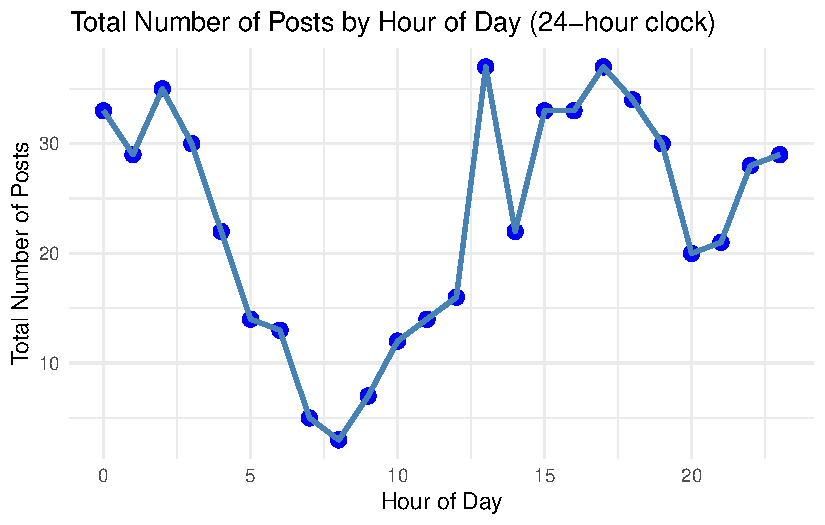
\includegraphics{Reddit_eda_files/figure-pdf/unnamed-chunk-6-1.pdf}

\begin{Shaded}
\begin{Highlighting}[]
\CommentTok{\# Number of comments by time of day (hour)}
\NormalTok{byhour\_comments }\OtherTok{\textless{}{-}}\NormalTok{ reddit\_comment }\SpecialCharTok{\%\textgreater{}\%}
  \FunctionTok{mutate}\NormalTok{(}\AttributeTok{hour\_of\_day =} \FunctionTok{hour}\NormalTok{(timestamp)) }\SpecialCharTok{\%\textgreater{}\%}
  \FunctionTok{group\_by}\NormalTok{(hour\_of\_day) }\SpecialCharTok{\%\textgreater{}\%}
  \FunctionTok{summarize}\NormalTok{(}\AttributeTok{total =} \FunctionTok{n}\NormalTok{())}

\CommentTok{\# Plot number of posts by hour of day}
\FunctionTok{ggplot}\NormalTok{(byhour\_comments, }\FunctionTok{aes}\NormalTok{(}\AttributeTok{x =}\NormalTok{ hour\_of\_day, }\AttributeTok{y =}\NormalTok{ total)) }\SpecialCharTok{+} 
  \CommentTok{\# geom\_bar(stat = "identity", fill = "lightgreen") + }
  \FunctionTok{geom\_point}\NormalTok{(}\AttributeTok{color =} \StringTok{"green"}\NormalTok{, }\AttributeTok{size =} \DecValTok{3}\NormalTok{) }\SpecialCharTok{+}  
  \FunctionTok{geom\_line}\NormalTok{(}\AttributeTok{color =} \StringTok{"lightgreen"}\NormalTok{, }\AttributeTok{linewidth =} \DecValTok{1}\NormalTok{) }\SpecialCharTok{+}
  \FunctionTok{labs}\NormalTok{(}
    \AttributeTok{title =} \StringTok{"Total Number of Comments by Hour of Day (24{-}hour clock)"}\NormalTok{,}
    \AttributeTok{x =} \StringTok{"Hour of Day"}\NormalTok{,}
    \AttributeTok{y =} \StringTok{"Total Number of Posts"}
\NormalTok{  ) }\SpecialCharTok{+}
  \FunctionTok{theme\_minimal}\NormalTok{()}
\end{Highlighting}
\end{Shaded}

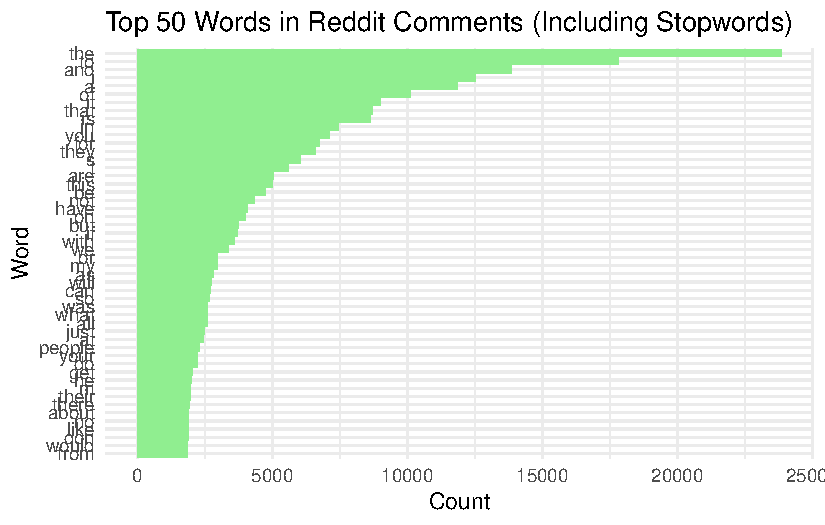
\includegraphics{Reddit_eda_files/figure-pdf/unnamed-chunk-6-2.pdf}

Most posts occur during the early morning, noon, and afternoon hours.
The highest peak is around lunchtime, likely due to people posting
during their lunch break. There is also significant activity in the
afternoon, evening, and early morning. This could be because people have
more free time or stay up late, allowing them to take the time to write
posts, which require more effort than quick interactions. The fewest
posts are seen in the morning, which makes sense as people are typically
getting ready for work, commuting, or sleeping in.

The trend for comments mirrors that of posts. This makes sense because
people are likely using Reddit at similar times for both posting and
commenting. However, the volume of comments is much higher than the
number of posts, as each post receives many comments from different
users.

\subsection{What are the words in the set of posts you have assembled
that appear most
frequently?}\label{what-are-the-words-in-the-set-of-posts-you-have-assembled-that-appear-most-frequently}

\begin{Shaded}
\begin{Highlighting}[]
\CommentTok{\# tokenize words to count frequencies for reddit posts}
\NormalTok{posts\_word\_counts }\OtherTok{\textless{}{-}}\NormalTok{ reddit\_posts }\SpecialCharTok{|\textgreater{}}
  \FunctionTok{select}\NormalTok{(title, text) }\SpecialCharTok{|\textgreater{}}
  \FunctionTok{pivot\_longer}\NormalTok{(}\AttributeTok{cols =} \FunctionTok{c}\NormalTok{(title, text), }\AttributeTok{values\_drop\_na =} \ConstantTok{TRUE}\NormalTok{) }\SpecialCharTok{|\textgreater{}}
  \FunctionTok{unnest\_tokens}\NormalTok{(word, value) }\SpecialCharTok{|\textgreater{}}
  \FunctionTok{count}\NormalTok{(word, }\AttributeTok{sort =} \ConstantTok{TRUE}\NormalTok{) }\SpecialCharTok{|\textgreater{}}
  \FunctionTok{slice\_max}\NormalTok{(n, }\AttributeTok{n =} \DecValTok{50}\NormalTok{)}

\CommentTok{\# plot}
\FunctionTok{ggplot}\NormalTok{(posts\_word\_counts, }\FunctionTok{aes}\NormalTok{(}\AttributeTok{x =} \FunctionTok{reorder}\NormalTok{(word, n), }\AttributeTok{y =}\NormalTok{ n)) }\SpecialCharTok{+}
  \FunctionTok{geom\_col}\NormalTok{(}\AttributeTok{fill =} \StringTok{"steelblue"}\NormalTok{) }\SpecialCharTok{+}
  \FunctionTok{coord\_flip}\NormalTok{() }\SpecialCharTok{+}
  \FunctionTok{labs}\NormalTok{(}\AttributeTok{title =} \StringTok{"Top 50 Words in Reddit Posts (Including Stopwords)"}\NormalTok{,}
       \AttributeTok{x =} \StringTok{"Word"}\NormalTok{,}
       \AttributeTok{y =} \StringTok{"Count"}\NormalTok{) }\SpecialCharTok{+}
  \FunctionTok{theme\_minimal}\NormalTok{()}
\end{Highlighting}
\end{Shaded}

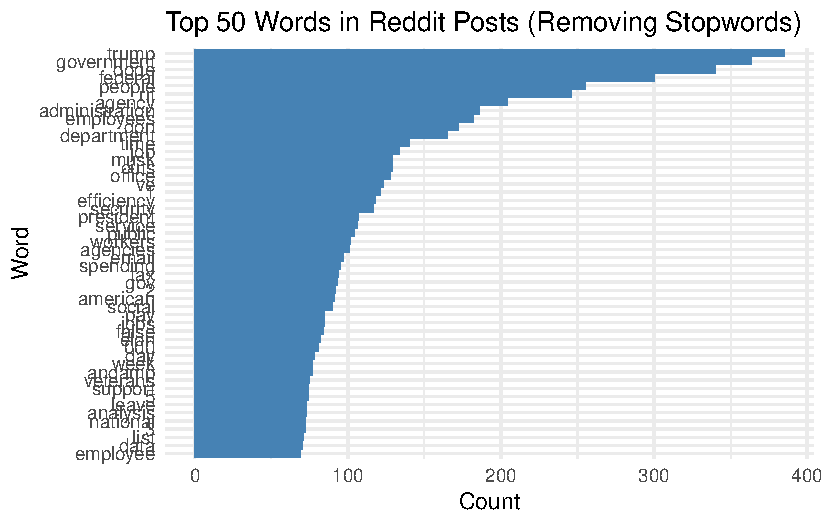
\includegraphics{Reddit_eda_files/figure-pdf/unnamed-chunk-7-1.pdf}

\begin{Shaded}
\begin{Highlighting}[]
\CommentTok{\# tokenize words to count frequencies for reddit comments}
\NormalTok{comments\_word\_counts }\OtherTok{\textless{}{-}}\NormalTok{ reddit\_comment }\SpecialCharTok{|\textgreater{}}
  \FunctionTok{select}\NormalTok{(comment) }\SpecialCharTok{|\textgreater{}}
  \FunctionTok{pivot\_longer}\NormalTok{(}\AttributeTok{cols =} \FunctionTok{c}\NormalTok{(comment), }\AttributeTok{values\_drop\_na =} \ConstantTok{TRUE}\NormalTok{) }\SpecialCharTok{|\textgreater{}}
  \FunctionTok{unnest\_tokens}\NormalTok{(word, value) }\SpecialCharTok{|\textgreater{}}
  \FunctionTok{count}\NormalTok{(word, }\AttributeTok{sort =} \ConstantTok{TRUE}\NormalTok{) }\SpecialCharTok{|\textgreater{}}
  \FunctionTok{slice\_max}\NormalTok{(n, }\AttributeTok{n =} \DecValTok{50}\NormalTok{)}

\CommentTok{\# plot}
\FunctionTok{ggplot}\NormalTok{(comments\_word\_counts, }\FunctionTok{aes}\NormalTok{(}\AttributeTok{x =} \FunctionTok{reorder}\NormalTok{(word, n), }\AttributeTok{y =}\NormalTok{ n)) }\SpecialCharTok{+}
  \FunctionTok{geom\_col}\NormalTok{(}\AttributeTok{fill =} \StringTok{"lightgreen"}\NormalTok{) }\SpecialCharTok{+}  \CommentTok{\# Removed extra parentheses}
  \FunctionTok{coord\_flip}\NormalTok{() }\SpecialCharTok{+}
  \FunctionTok{labs}\NormalTok{(}\AttributeTok{title =} \StringTok{"Top 50 Words in Reddit Comments (Including Stopwords)"}\NormalTok{,}
       \AttributeTok{x =} \StringTok{"Word"}\NormalTok{,}
       \AttributeTok{y =} \StringTok{"Count"}\NormalTok{) }\SpecialCharTok{+}
  \FunctionTok{theme\_minimal}\NormalTok{()}
\end{Highlighting}
\end{Shaded}

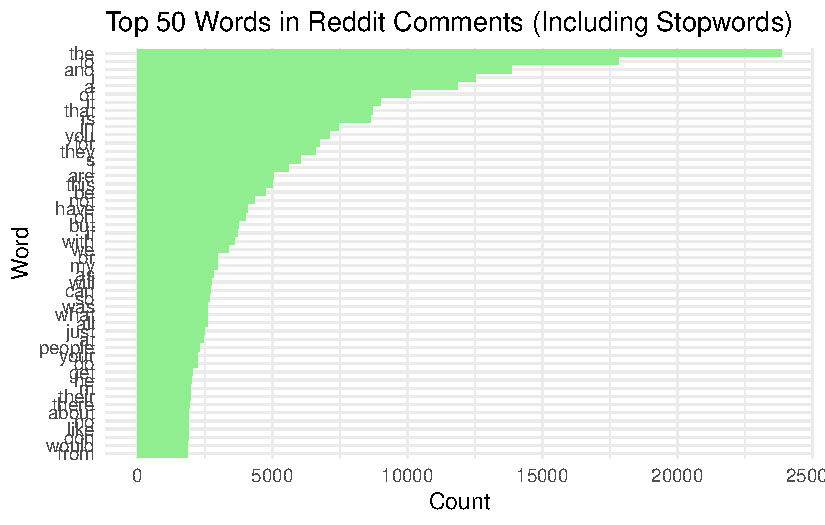
\includegraphics{Reddit_eda_files/figure-pdf/unnamed-chunk-7-2.pdf}

The graphs above show the most frequent words in both Reddit posts and
their comments. However, many of these words are stopwords, which don't
provide much insight into the actual content of the discussions. To get
a better understanding of what people are really talking about, we will
remove these stopwords in the next step.

\subsection{How does this change if you exclude ``stop words'' such as
``a,'' ``an,'' ``the,'' ``is,'' and others that are common in English
sentences but are generally not
informative?}\label{how-does-this-change-if-you-exclude-stop-words-such-as-a-an-the-is-and-others-that-are-common-in-english-sentences-but-are-generally-not-informative}

\begin{Shaded}
\begin{Highlighting}[]
\CommentTok{\# tokenize words to count frequencies for reddit posts removing stop words}
\NormalTok{posts\_word\_counts }\OtherTok{\textless{}{-}}\NormalTok{ reddit\_posts }\SpecialCharTok{|\textgreater{}}
  \FunctionTok{select}\NormalTok{(title, text) }\SpecialCharTok{|\textgreater{}}
  \FunctionTok{pivot\_longer}\NormalTok{(}\AttributeTok{cols =} \FunctionTok{c}\NormalTok{(title, text), }\AttributeTok{values\_drop\_na =} \ConstantTok{TRUE}\NormalTok{) }\SpecialCharTok{|\textgreater{}}
  \FunctionTok{unnest\_tokens}\NormalTok{(word, value) }\SpecialCharTok{|\textgreater{}}
  \FunctionTok{anti\_join}\NormalTok{(stop\_words, }\AttributeTok{by =} \StringTok{"word"}\NormalTok{) }\SpecialCharTok{|\textgreater{}}
  \FunctionTok{count}\NormalTok{(word, }\AttributeTok{sort =} \ConstantTok{TRUE}\NormalTok{) }\SpecialCharTok{|\textgreater{}}
  \FunctionTok{slice\_max}\NormalTok{(n, }\AttributeTok{n =} \DecValTok{50}\NormalTok{)}

\CommentTok{\# plot}
\FunctionTok{ggplot}\NormalTok{(posts\_word\_counts, }\FunctionTok{aes}\NormalTok{(}\AttributeTok{x =} \FunctionTok{reorder}\NormalTok{(word, n), }\AttributeTok{y =}\NormalTok{ n)) }\SpecialCharTok{+}
  \FunctionTok{geom\_col}\NormalTok{(}\AttributeTok{fill =} \StringTok{"steelblue"}\NormalTok{) }\SpecialCharTok{+}
  \FunctionTok{coord\_flip}\NormalTok{() }\SpecialCharTok{+}
  \FunctionTok{labs}\NormalTok{(}\AttributeTok{title =} \StringTok{"Top 50 Words in Reddit Posts (Removing Stopwords)"}\NormalTok{,}
       \AttributeTok{x =} \StringTok{"Word"}\NormalTok{,}
       \AttributeTok{y =} \StringTok{"Count"}\NormalTok{) }\SpecialCharTok{+}
  \FunctionTok{theme\_minimal}\NormalTok{()}
\end{Highlighting}
\end{Shaded}

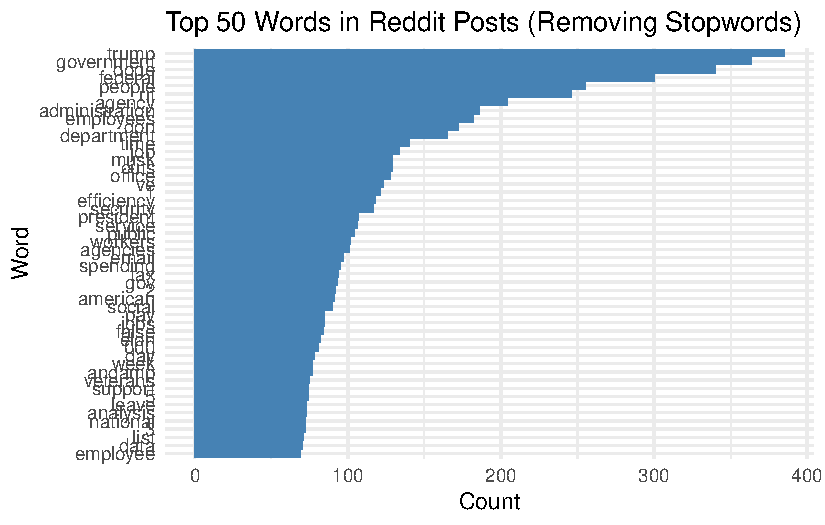
\includegraphics{Reddit_eda_files/figure-pdf/unnamed-chunk-8-1.pdf}

\begin{Shaded}
\begin{Highlighting}[]
\CommentTok{\# tokenize words to count frequencies for Reddit comments, removing stop words}
\NormalTok{comments\_word\_counts }\OtherTok{\textless{}{-}}\NormalTok{ reddit\_comment }\SpecialCharTok{|\textgreater{}}
  \FunctionTok{select}\NormalTok{(comment) }\SpecialCharTok{|\textgreater{}}
  \FunctionTok{pivot\_longer}\NormalTok{(}\AttributeTok{cols =} \FunctionTok{c}\NormalTok{(comment), }\AttributeTok{values\_drop\_na =} \ConstantTok{TRUE}\NormalTok{) }\SpecialCharTok{|\textgreater{}}
  \FunctionTok{unnest\_tokens}\NormalTok{(word, value) }\SpecialCharTok{|\textgreater{}}
  \FunctionTok{anti\_join}\NormalTok{(stop\_words, }\AttributeTok{by =} \StringTok{"word"}\NormalTok{) }\SpecialCharTok{|\textgreater{}}
  \FunctionTok{count}\NormalTok{(word, }\AttributeTok{sort =} \ConstantTok{TRUE}\NormalTok{) }\SpecialCharTok{|\textgreater{}}
  \FunctionTok{slice\_max}\NormalTok{(}\AttributeTok{order\_by =}\NormalTok{ n, }\AttributeTok{n =} \DecValTok{50}\NormalTok{)}

\CommentTok{\# plot}
\FunctionTok{ggplot}\NormalTok{(comments\_word\_counts, }\FunctionTok{aes}\NormalTok{(}\AttributeTok{x =} \FunctionTok{reorder}\NormalTok{(word, n), }\AttributeTok{y =}\NormalTok{ n)) }\SpecialCharTok{+}
  \FunctionTok{geom\_col}\NormalTok{(}\AttributeTok{fill =} \StringTok{"lightgreen"}\NormalTok{) }\SpecialCharTok{+}  \CommentTok{\# Removed extra parentheses}
  \FunctionTok{coord\_flip}\NormalTok{() }\SpecialCharTok{+}
  \FunctionTok{labs}\NormalTok{(}\AttributeTok{title =} \StringTok{"Top 50 Words in Reddit Comments (Removing Stopwords)"}\NormalTok{,}
       \AttributeTok{x =} \StringTok{"Word"}\NormalTok{,}
       \AttributeTok{y =} \StringTok{"Count"}\NormalTok{) }\SpecialCharTok{+}
  \FunctionTok{theme\_minimal}\NormalTok{()}
\end{Highlighting}
\end{Shaded}

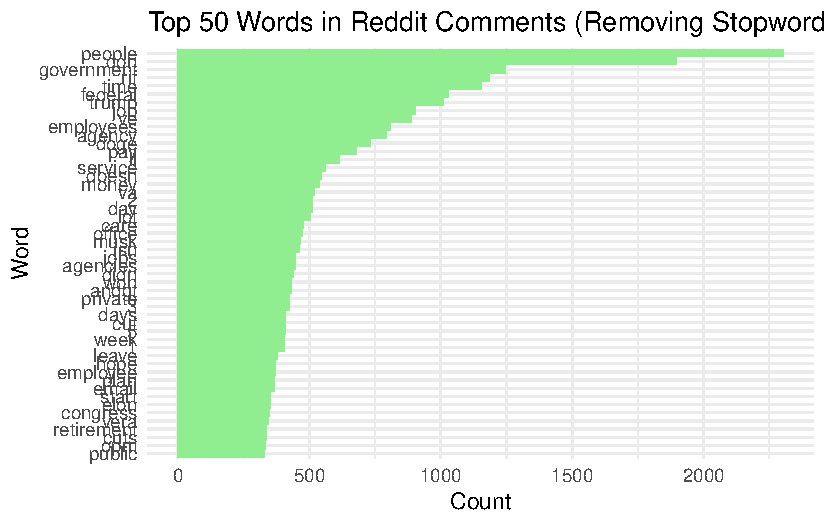
\includegraphics{Reddit_eda_files/figure-pdf/unnamed-chunk-8-2.pdf}

The graphs above show the most frequent words used in both Reddit posts
and their comment sections. We can see that many of these words are
directly related to our topic, with frequent mentions of the President,
DOGE, the federal government, and RIF.




\end{document}
